\documentclass[11pt]{article}
\usepackage[margin=1in]{geometry}
\usepackage{amsmath,amssymb}
\usepackage{graphicx}
\usepackage{booktabs}
\usepackage{siunitx}
\usepackage[hidelinks]{hyperref}
\usepackage{caption}
\captionsetup{font=small,labelfont=bf}
\sisetup{per-mode=symbol}

\title{Reinforcement learning versus an optimized forecast rule and an optimized fixed orifice
for the underdrain valve of a bioretention cell\\[4pt]
\large St.~Francis cell, conventional (30.2\,mm) footprint, perfect rainfall forecast}
\author{Arash Massoudieh\\ \small The Catholic University of America}
\date{Draft, 3 November 2026 (complete training runs)}

\begin{document}
\maketitle

\begin{abstract}
We compare three ways of operating the underdrain valve of a bioretention cell: a fixed
orifice of the best size, the forecast-informed rule of Gabbani et al.\ with its three
parameters optimized, and a reinforcement-learning (RL) policy trained with proximal policy
optimization (PPO) as an hourly correction on top of that rule. All three are optimized for
the same objective, using the same OpenHydroQual model, rainfall record (2020--2023) and
perfect forecast. Peak flow is measured as the outflow volume above a preset limit,
$\int \max(Q - Q_{\lim}, 0)\,dt$ with $Q_{\lim} = \SI{50}{\m^3\per\day}$, which is additive in
time, unlike the upper-tail statistic of the earlier study. Two objectives are considered:
the excess volume alone (case~1), and the excess volume plus the young-water load of an age
tracker, normalized by the passive cell and weighted equally (case~2). In case~1 the
optimized rule ($J = 0.0768$) beats the best fixed orifice ($0.0889$) by 14\%, and PPO does
not improve on the rule: after 3 million training steps the final policy scores 0.0831,
and no trained checkpoint beats the rule. In case~2 the rule ($J = 0.285$) beats the
orifice ($0.426$) by 33\%, and the final PPO policy beats the rule by a further 10\%
($J = 0.256$; checkpoints late in training reach 0.186): it keeps the cell three times
fuller on average, cutting the young-water load by 43\%, at the cost of 60\% more excess
volume. These are in-sample results. Trained on 2020--2022 and tested on 2023, a dry year
with no flow above the limit, the case-2 policy keeps a third of the rule's young-water
load. With 2020 held out (rule and orifice re-tuned and PPO
retrained on 2021--2023), the case-2 gain holds on the unseen year: PPO scores $J = 0.447$
on 2020 against $0.673$ for the rule (34\% lower) and $0.894$ for the orifice, lowering both
the excess and the young-water load. In case~1 PPO is again slightly worse than the rule on
2020 (0.200 against 0.189).
\end{abstract}

\section{Introduction}
Forecast-informed real-time control of a bioretention underdrain can lower outflow peaks
by releasing water ahead of a storm and holding it otherwise. Gabbani et al.\ proposed a
three-parameter rule: the valve opens in proportion to the square root of a kernel-smoothed
rainfall forecast and closes when that forecast is below a threshold. The later
forecast-uncertainty study found that, once the overflow weir is realistic and the time step
converged, this rule beats a well-sized fixed orifice only modestly on peak flow, but by
30--40\% when residence time is also rewarded.

Here we ask whether a learned policy can do better than the rule when both have the same
information (a perfect forecast) and the same objective. To make the comparison fair, the
rule and the fixed orifice are both re-optimized on the objective used to train the RL
policy, and all three are scored on the same whole-record runs.

\section{System and model}
The model is the St.\ Francis bioretention cell of the forecast-uncertainty study at half
of its as-built plan area: \SI{30.2}{mm} of storage over the \SI{7300}{\m^2} catchment, the
conventional water-quality sizing, where that study found forecast control most valuable.
Runoff from four catchment segments enters a pond (crest \SI{158.2}{m}, 1\,m sharp-crested
weir to the catch basin), infiltrates through the engineered media into an aggregate
storage layer, and leaves either to the native soil or through the controlled underdrain
(diameter \SI{0.2}{m}) to the catch basin. The catch-basin outflow pipe, carrying both the
weir overflow and the underdrain flow, is where all objectives are measured. Forcing is the
hourly 2020--2023 record (precipitation, and temperature, humidity, radiation and wind for
Penman evapotranspiration). A Laplace age tracker (unit concentration on every inflow,
first-order decay $\lambda = \SI{1}{\per\day}$) carries $E[e^{-\lambda\,\mathrm{age}}]$, so its
exported load is the \emph{young-water load}: lower means water is held longer.

The model files are the study's residence-time models
(\url{rt_campaign/models/R1_f0.50_half_30.2mm/sigma_0_ts_2}) and its passive
reference, with only three changes: the objectives are replaced (Section~\ref{sec:obj}), the
templates are read from the current OpenHydroQual master (whose changes since the pinned
commit only add new types), and, for the fixed orifice and the RL policy, the valve is
replaced by a controlled orifice (below). Numerics are the study's: initial step
\SI{0.01}{d}, maximum step \SI{0.1}{d}.

\section{Objectives}\label{sec:obj}
Both objectives are integrals over the record, so they are additive in time and can serve
directly as an RL reward:
\begin{align}
\mathrm{Excess} &= \int_{t_0}^{t_1} \max\!\big(Q(t) - Q_{\lim},\,0\big)\,dt,
  \qquad Q_{\lim} = \SI{50}{\m^3\per\day}\ (\SI{0.58}{L/s}),\\
\mathrm{Age} &= \int_{t_0}^{t_1} Q(t)\,c_{\mathrm{age}}(t)\,dt,
\end{align}
where $Q$ is the catch-basin outflow and $c_{\mathrm{age}}$ the age-tracer concentration. The
limit was chosen between the rule's typical release rate (50--80\,\si{\m^3\per\day}) and the
passive cell's 99th-percentile outflow (about \SI{100}{\m^3\per\day}). Each term is normalized
by the passive cell (valve replaced by a free-draining underdrain): Excess$_p$ =
\SI{2793}{\m^3}, Age$_p$ = 2753. The two cases are
\begin{align}
\text{case 1:}\quad J_1 &= \mathrm{Excess}/\mathrm{Excess}_p, \\
\text{case 2:}\quad J_2 &= \mathrm{Excess}/\mathrm{Excess}_p + \mathrm{Age}/\mathrm{Age}_p,
\end{align}
so the passive cell scores 1 and 2. Lower is better.

\section{Controllers}
\paragraph{Fixed orifice.} The controlled-orifice link has the same head dependence as the
valve, $Q_v = 86400\,u\,A\sqrt{2g}\,\Delta h/\sqrt{\Delta h + \SI{1}{mm}}$, with $A$ the
valve area and $u$ the opening. The best constant $u$ is found by a sweep of 48 sizes
(geometric, $2\times10^{-4}$ to $0.05$) for each case.

\paragraph{Forecast rule.} With a perfect forecast the rule is
\begin{equation}
u_{\mathrm{rule}}(t) = \begin{cases}\sqrt{\hat I(t)/S} & \hat I(t) > I_0\\ 0 & \text{otherwise},\end{cases}
\end{equation}
where $\hat I$ is the rainfall rate $r$ convolved with a truncated, forward-looking
exponential kernel:
\begin{equation}
\hat I(t) = \int_{0}^{2\tau_k} K(\tau)\, r(t+\tau)\, d\tau = (\tilde K * r)(t),
\qquad K(\tau) = \lambda_k\, e^{-\lambda_k \tau},\quad \lambda_k = 1/\tau_k,
\label{eq:ihat}
\end{equation}
with $\tilde K(\tau) = K(-\tau)$, so the convolution looks ahead in time: with a perfect
forecast, $\hat I(t)$ weighs the rain of the next $2\tau_k$ days, most heavily the rain
closest to $t$. The kernel is truncated at two time constants, where it keeps
$1-e^{-2} \approx 86\%$ of its weight. OpenHydroQual evaluates~\eqref{eq:ihat} on the
rainfall series $(t_i, r_i)$ by the trapezoidal rule,
$\hat I(t) = \sum_i r_i\,\lambda_k\,\tfrac12\big(e^{-\lambda_k (t_i - t)} + e^{-\lambda_k
(t_{i+1}-t)}\big)(t_{i+1}-t_i)$, and the controller here uses this sum exactly as the model
does.\footnote{Versions of OpenHydroQual before 2 November 2026 omitted the $\tfrac12$,
doubling $\hat I$. Because $\hat I$ enters the rule only through $\hat I/S$ and the
comparison with $I_0$, this is equivalent to halving $S$ and $I_0$: the same controller,
the same $J$. All parameters here are given for the corrected kernel; parameters tuned with
the earlier version convert as $S \to S/2$, $I_0 \to I_0/2$.} The three parameters $(S, I_0, \tau_k)$ are optimized by CMA-ES in log
space (population 12, 35 generations, bounds $S\in[5,2000]$,
$I_0\in[5\times10^{-7},0.015]$\,m/d, $\tau_k\in[0.001,100]$\,d), separately for each case, starting
from the better of the study's two perfect-forecast optima. Re-tuning lowered $J$ by 34\%
(case~1) and 23\% (case~2) relative to those starting points, so the study's parameters,
tuned for a different peak statistic, would have been a weak benchmark. The rule is scored
in its own model, where the valve responds to $\hat I$ continuously.

\paragraph{PPO.} The RL policy corrects the rule every hour:
$u = \mathrm{clip}(u_{\mathrm{rule}} + a\,u_s,\ 0,\ 0.03)$ with $a\in[-1,1]$ and
$u_s = 0.004$, so $a = 0$ is the rule applied hourly. The observation (16 values) holds the
ponded, aggregate-layer, media and catch-basin storages, the outflow and weir flow, the
rule's opening, the perfect-forecast mean rainfall over the next 0--3\,h, 3--12\,h,
12--24\,h, 1--3\,d and 3--7\,d, the past day's rainfall, $\hat I$, and the season. The reward
is minus the increase of $J$ over the hour, so the return of an episode is minus its $J$.
Episodes are 30-day windows starting at random times in the record, each initialized from
the state of a continuous run of the hourly rule at that time. Training: actor-critic with
two hidden layers of 64 (tanh), PPO with GAE ($\gamma = 0.995$, $\lambda = 0.95$, clip 0.2,
10 epochs, minibatch 1024, learning rate $3\times10^{-4}$), 6 workers $\times$ 720 steps per
update (4,320 steps; 694 updates, 3 million steps, one seed per case), reward normalization, and the actor first cloned to $a = 0$ (the rule) with
exploration $\log\sigma = -1.2$. Checkpoints every 20 updates were scored deterministically
over the whole record. The policy reported is the final one; the checkpoints show how
much the result depends on where training stops.

\section{Simulation and verification}
Each controller is simulated with a compiled OpenHydroQual kernel (\texttt{ohq\_generate}),
driven from Python: the opening is a kernel parameter set before each hour, and the
objectives are integrated from the kernel's per-step series as OpenHydroQual integrates
them. A whole-record run takes about \SI{12}{s} (more than 18 minutes interpreted), and a
30-day training episode \SI{0.4}{s}. Three checks:
\begin{itemize}
\item The hourly rule on the orifice model reproduces the rule model to within 0.2\% (case~1)
and 0.6\% (case~2) in $J$; the remaining difference is that the native valve switches within
the hour.
\item An episode started from a stored state reproduces the continuous run over the same
window to 0.01\%.
\item Storages of the compiled kernel match the interpreted model to 0.1\% over a 30-day
test with a switching opening.
\end{itemize}

\section{Results}
\begin{table}[t]
\centering\small
\caption{Whole-record (2020--2023) results with a perfect forecast. Excess in
\si{\m^3}; peak outflow in \si{\m^3\per\day}; hours with outflow above $Q_{\lim}$; weir
overflow volume in \si{\m^3}. PPO is the final policy (update 694) of each training run.}
\label{tab:main}
\begin{tabular}{lrrrrrrr}
\toprule
 & $J$ & Excess & Excess/Ex$_p$ & Age/Age$_p$ & Peak & Hours $>Q_{\lim}$ & Weir vol.\\
\midrule
\multicolumn{8}{l}{\emph{Case 1: excess only}}\\
Passive (free draining) & 1.000 & 2793 & 1.000 & 1.000 & 755 & 1156 & 0\\
Best fixed orifice & 0.089 & 248 & 0.089 & 0.451 & 526 & 80 & 259\\
Tuned forecast rule & 0.077 & 215 & 0.077 & 0.327 & 266 & 195 & 140\\
PPO (final policy) & 0.083 & 232 & 0.083 & 0.243 & 374 & 180 & 357\\
\addlinespace
\multicolumn{8}{l}{\emph{Case 2: excess + residence time}}\\
Passive (free draining) & 2.000 & 2793 & 1.000 & 1.000 & 755 & 1156 & 0\\
Best fixed orifice & 0.426 & 364 & 0.130 & 0.295 & 632 & 135 & 570\\
Tuned forecast rule & 0.285 & 255 & 0.091 & 0.194 & 489 & 214 & 502\\
PPO (final policy) & 0.256 & 407 & 0.146 & 0.111 & 354 & 262 & 754\\
\addlinespace
\bottomrule
\end{tabular}
\end{table}

\begin{table}[t]
\centering\small
\caption{Optimized parameters.}
\label{tab:params}
\begin{tabular}{lccc|c}
\toprule
 & \multicolumn{3}{c|}{Forecast rule} & Fixed orifice\\
 & $S$ & $I_0$ (m/d) & $\tau_k$ (d) & opening $u$\\
\midrule
Case 1 & 272 & $1.6\times10^{-6}$ & 4.49 & 0.00377\\
Case 2 & 804 & $5.0\times10^{-7}$ (bound) & 1.95 & 0.00210\\
\bottomrule
\end{tabular}
\end{table}

\begin{figure}[t]
\centering
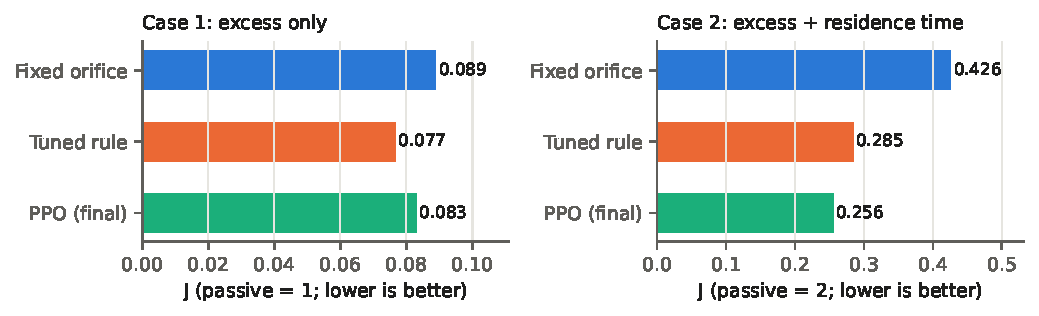
\includegraphics[width=\linewidth]{figures/J_bars.pdf}
\caption{Objective $J$ of the three optimized controllers over the whole record.}
\label{fig:bars}
\end{figure}

\paragraph{Case 1: excess only.} The optimized rule beats the best fixed orifice by 14\%
(Table~\ref{tab:main}, Figure~\ref{fig:bars}). It halves the peak outflow (266 against
\SI{526}{\m^3\per\day}) and the weir overflow (140 against \SI{259}{\m^3}), although it
exceeds the limit for more hours (195 against 80): it releases more, at moderate rates,
before storms. PPO does not improve on it. After an early excursion (up to 0.233 at update
60) training settles close to the rule, between 0.077 and 0.084 from update 300 on
(Figure~\ref{fig:training}), but no trained checkpoint beats the starting policy, the hourly
rule ($J = 0.0767$). The final policy scores 0.0831, 8\% worse than the rule. It holds more
water than the rule (\SI{14.9}{\m^3} ponded on average against \SI{5.2}{\m^3}, valve shut
24\% of the time), which lowers the hours above the limit (180 against 195) and, as a side
effect, the young-water load (0.243 against 0.327), but raises the peak (374 against
\SI{266}{\m^3\per\day}) and the weir overflow (357 against \SI{140}{\m^3}).

\paragraph{Case 2: excess plus residence time.} The rule beats the fixed orifice by 33\%:
it is lower on both terms (excess 0.091 against 0.130, young-water load 0.194 against
0.295 of passive), which no single orifice size achieves (Figure~\ref{fig:tradeoff}; the orifice sizes trace a curve that the rule lies well
inside). The final PPO policy beats the rule by a further 10\% ($J = 0.256$). It reaches
this by a different balance (Figure~\ref{fig:tradeoff}): the young-water load falls by 43\%
(0.111 against 0.194 of passive) while the excess rises by 60\% (0.146 against 0.091). The
policy keeps the valve shut 37\% of the time (the hourly rule 26\%), keeps on average
\SI{58}{\m^3} ponded against \SI{17}{\m^3}, and so overflows the weir more (754 against
\SI{502}{\m^3}) and exceeds the limit for more hours (262 against 214), while lowering the
peak outflow (354 against \SI{489}{\m^3\per\day}).

Where training stops matters (Figure~\ref{fig:training}). The first 140 updates are worse
than the rule, up to $J = 1.45$ at update 60, worse than the passive cell, as the policy
leaves the rule. From update 160 on, all 28 checkpoints are better than the rule, with a
median of 0.214 (25\% below the rule) and a range of 0.186 to 0.262. The best, update 620 ($J = 0.186$, 35\% below the rule), is
lower than the rule on both terms (excess 0.103, young-water load 0.083), so a better balance
than the final policy's exists. The final policy is near the upper end of this range;
training does not converge to a single policy, and the gain at any one stopping point
varies between about 10\% and 35\%.

\begin{figure}[t]
\centering
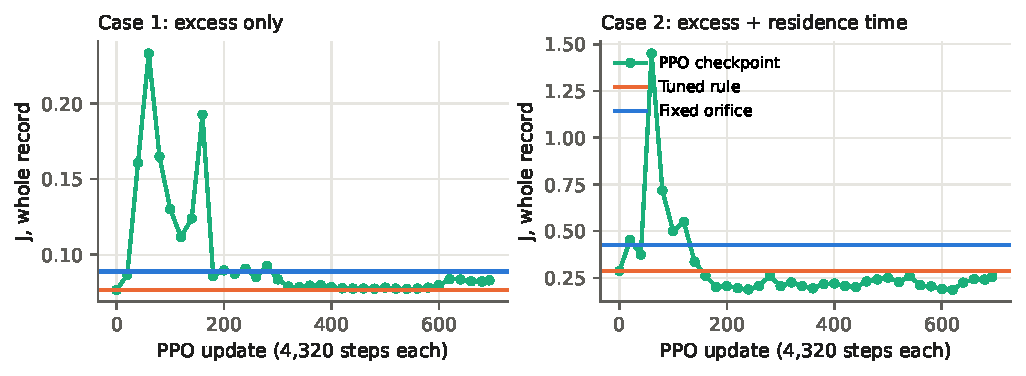
\includegraphics[width=\linewidth]{figures/training.pdf}
\caption{Whole-record $J$ of the PPO checkpoints (update 0 is the rule applied hourly).
The last point is the final policy (update 694, 3 million steps).}
\label{fig:training}
\end{figure}

\begin{figure}[t]
\centering
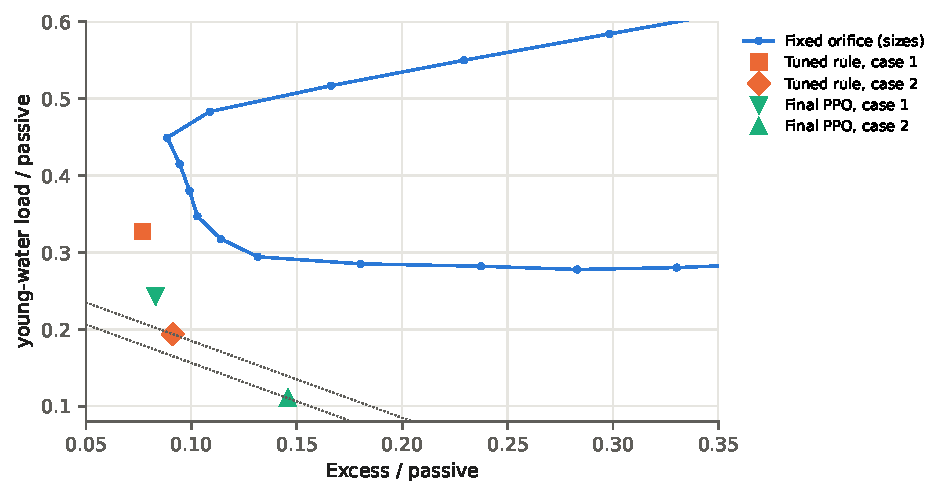
\includegraphics[width=0.9\linewidth]{figures/tradeoff.pdf}
\caption{Excess and young-water load (both relative to passive). The fixed orifice traces a
curve as its size varies; dotted lines are lines of equal case-2 $J$ through the rule and the
final PPO policy (case~2).}
\label{fig:tradeoff}
\end{figure}

\begin{figure}[t]
\centering
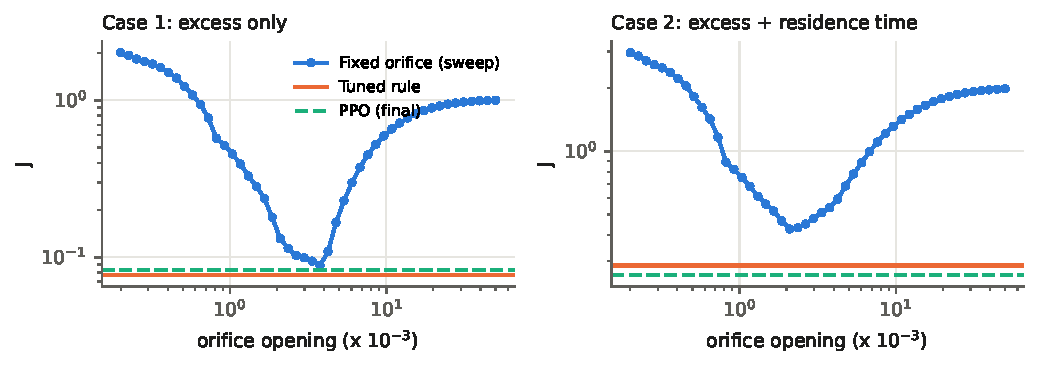
\includegraphics[width=\linewidth]{figures/orifice_sweep.pdf}
\caption{$J$ of the fixed orifice against its opening, with the optimized rule and the final PPO
policy.}
\label{fig:sweep}
\end{figure}

\paragraph{The largest storm.} In the largest 24-hour storm of the record
(Figure~\ref{fig:storm}), all controlled cells fill to about \SI{200}{\m^3} and overflow;
the differences are before and after the storm. The rule and the case-2 PPO policy open
ahead of the storm as the forecast rises, which the fixed orifice cannot; PPO opens slightly
less (mean opening $5.1\times10^{-3}$ over the three days before the storm against
$5.8\times10^{-3}$). As the storm peaks, PPO almost closes the valve (opening
$0.4\times10^{-3}$, against the rule's minimum of $1.5\times10^{-3}$), and then, over the
following days, opens it wider than the rule (mean $3.5\times10^{-3}$ against
$3.0\times10^{-3}$), so the cell is drained further by the end of the window (134 against
\SI{152}{\m^3}). In this storm PPO holds water at the peak and releases it afterwards.

\begin{figure}[t]
\centering
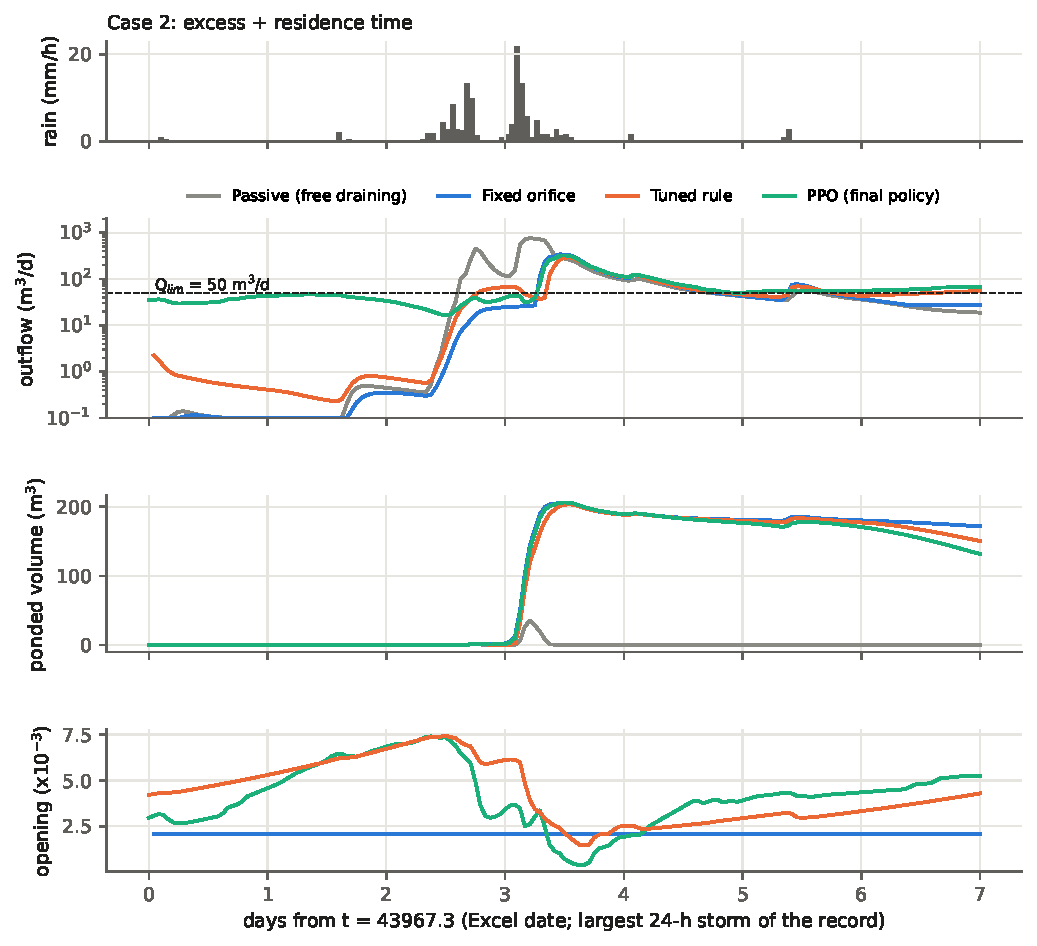
\includegraphics[width=\linewidth]{figures/storm_R1.pdf}
\caption{Largest 24-hour storm, case-2 controllers: rainfall, outflow (log scale, with
$Q_{\lim}$), ponded volume and valve opening (the rule's opening is shown applied hourly).}
\label{fig:storm}
\end{figure}

\subsection{Held-out year: 2023}\label{sec:test2023}
The first test held out the last year: the passive reference, orifice sweep, rule tuning,
snapshots and PPO training were redone on 2020--2022, and each controller was scored on 2023
(same protocol as for 2020 below). The re-tuned rule and orifice are essentially those of
the whole record (case~1: $S = 273$, $I_0 = 6.6\times10^{-6}$, $\tau_k = 4.48$, orifice 0.00377;
case~2: $S = 800$, $I_0 = 5.0\times10^{-7}$, $\tau_k = 1.96$, orifice 0.00210), since 2023 adds
no excess. 2023 is dry: the passive cell exceeds the limit by only \SI{346}{\m^3}, and no
controlled cell exceeds it at all. In case~1 every controller therefore scores $J = 0$ on
2023 and the test cannot separate them. In case~2 only the young-water load is left: the
final PPO policy scores 0.051 against 0.155 for the rule and 0.293 for the orifice, a third
of the rule's load, consistent with its in-sample behaviour of holding water longer. On the
training years it scores 0.249 against the rule's 0.305. A year with large storms is needed
to test the excess term out of sample, hence the 2020 test.

\subsection{Held-out year: 2020}\label{sec:holdout}
To test whether the gains carry over to storms the controllers have not seen, 2020, the
wettest year, was held out. Everything was redone on 2021--2023 alone: the passive reference, the orifice sweep,
the CMA-ES tuning of the rule, the snapshots and the PPO training (episodes start only in
2021--2023; 3 million steps, 694 updates of 6 workers $\times$ 720 steps, one seed). Each
controller is then run over the whole 2020--2023 record under its own control, and the
integrals are split at 1 January 2021, so the 2020 score starts from the state the
controller itself produced. Both windows are normalized by the passive cell in the same
window (2020: Excess$_p$ = \SI{1177}{\m^3}, Age$_p$ = 990; 2021--2023: \SI{1617}{\m^3} and
1763). The PPO policy reported is the final one, chosen without looking at 2020. The re-tuned
parameters are $(S, I_0, \tau_k) = (398,\ 5.0\times10^{-7}\text{ (bound)},\ 3.00)$ and orifice
opening 0.00236 for case~1, and $(1470,\ 1.6\times10^{-6},\ 3.47)$ and 0.00166 for case~2.

2020 is the wettest year of the record: it holds 42\% of the passive excess volume of the
four years. 2021--2023 has almost no flow above the limit once the cell is controlled. In
case~1 the rule and the orifice have no excess at all on the training years ($J = 0$), so
there is nothing for PPO to improve and nothing to choose between the two benchmarks there.

\begin{table}[t]
\centering\small
\caption{Held-out year. Controllers tuned or trained on 2021--2023, scored on 2021--2023
and on 2020, each relative to the passive cell in that window. Excess in \si{\m^3}. PPO is
the final policy (update 694). In case~1 Age/Age$_p$ is not part of $J$ and is shown for
reference.}
\label{tab:holdout}
\begin{tabular}{lrrrrr}
\toprule
 & $J$, 2021--23 & $J$, 2020 & Excess, 2020 & Ex/Ex$_p$, 2020 & Age/Age$_p$, 2020\\
\midrule
\multicolumn{6}{l}{\emph{Case 1: excess only}}\\
Best fixed orifice & 0.000 & 0.264 & 311 & 0.264 & 0.343\\
Tuned forecast rule & 0.000 & 0.189 & 222 & 0.189 & 0.308\\
PPO (final) & 0.005 & 0.200 & 236 & 0.200 & 0.408\\
\addlinespace
\multicolumn{6}{l}{\emph{Case 2: excess + residence time}}\\
Best fixed orifice & 0.247 & 0.894 & 595 & 0.506 & 0.389\\
Tuned forecast rule & 0.130 & 0.673 & 438 & 0.373 & 0.301\\
PPO (final) & 0.049 & 0.447 & 311 & 0.265 & 0.182\\
\bottomrule
\end{tabular}
\end{table}

\begin{figure}[t]
\centering
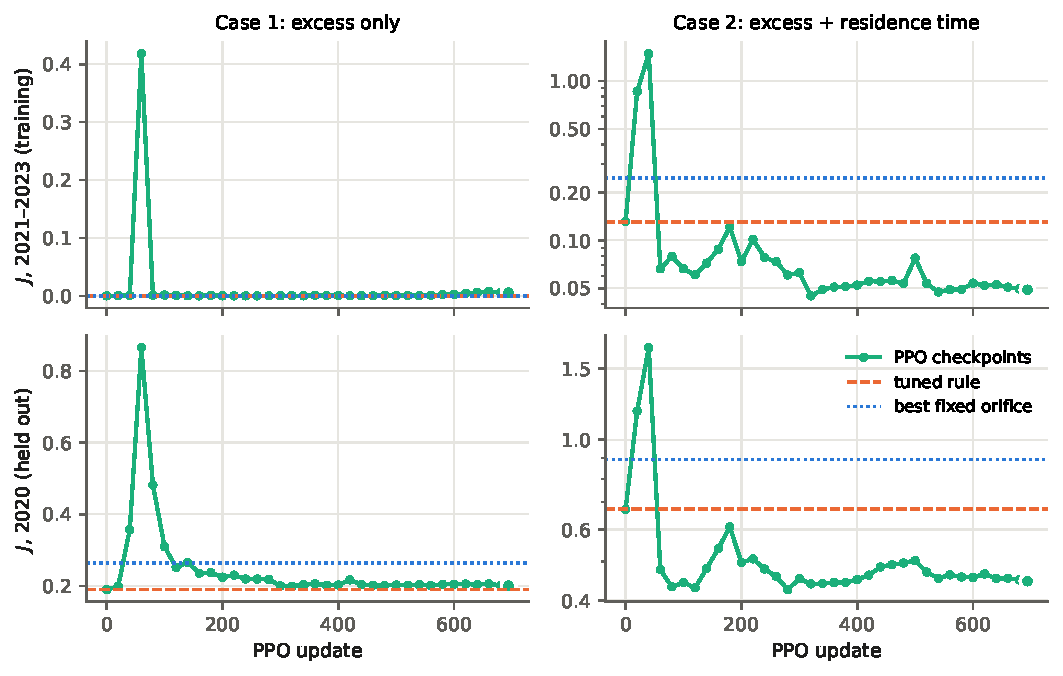
\includegraphics[width=\linewidth]{figures/holdout_2020.pdf}
\caption{Held-out test. $J$ of every PPO checkpoint (trained on 2021--2023) on the training
years (top) and on 2020 (bottom), with the rule and orifice tuned on 2021--2023. The large
dot is the final policy. Case~2 is on a log scale.}
\label{fig:holdout}
\end{figure}

\paragraph{Case 2.} The ranking of the in-sample results holds on 2020
(Table~\ref{tab:holdout}). The rule beats the orifice by 25\% (0.673 against 0.894), and the
final PPO policy beats the rule by 34\% ($J = 0.447$). Unlike the in-sample policy, it does
so on both terms: 29\% less excess volume (311 against \SI{438}{\m^3}) and 39\% less
young-water load (0.182 against 0.301 of passive). The gain is not a matter of picking a
lucky checkpoint (Figure~\ref{fig:holdout}). After a transient in the first 40 updates, when
the policy first leaves the rule and is worse than the orifice, every one of the 32
checkpoints from update 80 to 694 is better than the rule on 2020, between 0.426 and 0.609;
the checkpoint best on the training years (update 320, $J = 0.045$) scores 0.440 on 2020,
close to the final policy. The gain is smaller on 2020 than on the training years (63\%),
as expected out of sample, but it is larger than the 10\% gain of the final in-sample
policy, and within the 10--35\% range of the in-sample checkpoints.

\paragraph{Case 1.} PPO does not beat the rule on 2020 either: the final policy scores
0.200 against 0.189 (6\% worse), still well ahead of the orifice (0.264). Since the training
years give it almost no excess to reduce, the policy drifts towards holding water (its
young-water load is 0.408, against 0.308 for the rule), which costs it a little excess in
2020. No case-1 checkpoint after update 0 beats the rule on 2020.

\section{Discussion and limitations}
The results repeat the pattern of the forecast-uncertainty study. When only high flows
count, the optimized rule already captures most of what the forecast offers, and PPO finds
nothing better. When residence time also counts, there is a balance between holding and
releasing water that a rule driven only by the forecast does not express well, and PPO,
which also sees the storages, finds a better one. The case-2 result rests on the following
qualifications.
\begin{enumerate}
\item \textbf{In-sample.} As in the study's GA campaign, all controllers are tuned and scored
on the same 2020--2023 record, and a gain from a 4,500-parameter network may partly reflect
the particular storms of the record. The hold-out tests answer this in part: trained and
tuned without 2020, PPO beats the rule on 2020 by 34\% in case~2 (Section~\ref{sec:holdout}),
and trained without 2023 it keeps a third of the rule's young-water load in that dry year
(Section~\ref{sec:test2023}). Each is one year and one seed, however, and the training years contain almost no flow
above the limit under control, so the excess term contributes little to the training
signal; a held-out year with fewer large storms might not show the same gain.
\item \textbf{Single, unconverged training runs.} Each policy is one seed of 3 million steps.
The case-2 checkpoints keep moving between $J = 0.186$ and 0.262 late in training, so the
gain over the rule depends on where training stops (10\% for the final policy, 35\% for
the best checkpoint), and the final policy is not the best one. Repeated seeds, and a
stopping rule chosen on a validation period, would make the reported gain less arbitrary.
\item \textbf{Rule optimum.} Each rule was tuned by one CMA-ES run, and in case~2 the
threshold sits on its lower bound. Restarts and a wider bound would confirm that the rule
is at its best within its form.
\item \textbf{Perfect forecast and hourly decisions.} With forecast error the rule's
advantage over the orifice shrinks, especially in larger cells; how a learned policy
degrades is untested. The policy acts hourly, while the native rule responds continuously
(which costs it nothing here: the hourly rule scores within 0.6\%).
\item \textbf{The limit $Q_{\lim}$} was set at \SI{50}{\m^3\per\day}; other limits, or a
nonlinear function of the excess, weight the peaks differently and may change the ranking.
\end{enumerate}

\section{Conclusions}
\begin{itemize}
\item With the excess volume above \SI{50}{\m^3\per\day} as the objective, the optimized
forecast rule beats the best fixed orifice by 14\%, and PPO cannot improve on the rule, in
sample or on the held-out year 2020.
\item With excess volume and residence time weighted equally, the rule beats the orifice by
33\%, and PPO beats the rule by a further 10\% in sample with its final policy (25\% at
the median late checkpoint), mainly by holding water longer.
\item The case-2 gain holds out of sample: trained and tuned on 2021--2023, PPO beats the
rule by 34\% on the held-out year 2020, lowering both the excess volume and the young-water
load; on the dry held-out year 2023 it keeps a third of the rule's young-water load.
Repeated seeds and a principled stopping rule are still needed.
\end{itemize}

\appendix
\section{Reproducing}
\sloppy
All code is in \texttt{OpenHydroQual-RL/stfrancis}: \texttt{build\_models.py} (models),
kernels via \texttt{ohq\_generate}, \texttt{tune\_rule.py} (passive reference, orifice sweep,
CMA-ES rule tuning), \texttt{snapshots.py}, \texttt{sf\_env.py} (environment),
\texttt{../train\_ppo.py --env stfrancis}, \texttt{evaluate\_sf.py} and
\texttt{make\_paper.py}; \texttt{run\_rl.sh} chains the RL steps. The hold-out test is
\texttt{campaign\_split.sh ho2020} (tuning, snapshots, training and scoring on 2021--2023
with 2020 held out) and \texttt{make\_holdout.py} (Figure~\ref{fig:holdout}).

\end{document}
